\chapter{无约束光滑目标的求解}
\label{chap:smooth-optimization}

本章只考虑无约束、目标可微的优化问题。有了第10章可判定的最优性条件，还需构造能逐步接近它的参数序列。为了把不同方法放在同一把尺子下比较，本章反复使用
\begin{equation}
 f(\bm w)=\frac12(w_1^2+16w_2^2),\qquad
 \bm H=\operatorname{diag}(1,16),\qquad
 \bm w^{(0)}=(2,2)^\top.
 \label{eq:opt-common-quadratic}
\end{equation}
它的最小点为零，初始目标值为$34$，两个坐标方向的曲率相差$16$倍，使每种方法的方向、步长和每步成本都能直接核算。

本章的前半介绍方法，后半回答四个共同问题。11.1节从梯度及历史形成方向：普通梯度下降、固定预条件、动量与符号方向、逐坐标历史缩放，以及矩阵方向变换；11.2节用局部模型给出候选步：牛顿族、Gauss--Newton族、拟牛顿，以及按模型输出变化度量位移的自然梯度；11.3节处理学习率、参数衰减和执行次序。方向构造、模型求解与更新控制是三种可组合的职责，而不是互斥的算法类别。11.4节比较收敛速度与计算成本，11.5节分析数值误差传播和最优解对扰动的敏感性，11.6节讨论非最小驻点与逃离鞍点，11.7节解释优化路径在多解问题中的隐式偏置。

阅读方法部分时应能据输入写出一轮更新并说出返回什么；性质部分再判断下降、收敛速度、计算量与解的选择。平方梯度的非中心二阶矩不是目标Hessian，矩阵乘法也不自动意味着使用了二阶信息。抽样与小批量在第14章讨论；本章的梯度都是同一明确目标的真实梯度。

\section{基于梯度的方向构造}
\label{sec:opt-first-order-methods}

本节回答“怎样把当前及历史梯度变成一个可执行方向”。统一记第$t$轮参数为$\bm w^{(t)}$、$\bm g^{(t)}=\nabla f(\bm w^{(t)})$，逐坐标向量运算以$\odot$表示逐元素乘法。给定预算和精度标准后，方法返回实际参数点及所需历史状态；停止时核验原目标或真实梯度，不能把平滑后方向小、步长缩小或参数位移小当作证书。

\subsection{梯度下降与回溯步长}
\label{sec:opt-gradient-descent}

对可求梯度的有限维实值目标$f:\mathbb R^d\to\mathbb R$，梯度给出当前点最陡的上升方向，梯度下降取其反向：
\begin{equation}
  \bm{w}^{(t+1)}=\bm{w}^{(t)}-\eta^{(t)}\nabla f(\bm{w}^{(t)}).
  \label{eq:opt-gradient-descent}
\end{equation}
沿负梯度走“足够小”的一步一定下降：函数值变化的一阶近似为$-\eta\|\nabla f\|_2^2<0$。问题在于“足够小”没有可事先使用的尺度；位移越大，被舍弃的高阶项影响越大。要把它换成可计算的步长范围，需要控制移动后梯度改变多少。

\begin{definition}[欧氏梯度光滑性]
\label{def:opt-smoothness}
设$f:\mathbb R^d\to\mathbb R$可微，$L\geq0$有限。若对任意$\bm u,\bm v$都有
$\lVert\nabla f(\bm{u})-\nabla f(\bm{v})\rVert_2
\leq L\lVert\bm{u}-\bm{v}\rVert_2$，
则称$f$为\term{$L$光滑}（$L$-smooth）。
\end{definition}

常数$L$给“每移动单位距离，梯度最多改变多少”定了上限。沿线段积分即可得到控制一阶模型余项的下降引理。

\begin{lemma}[下降引理]
\label{lem:opt-descent}
若$f$可微且梯度是$L$-Lipschitz连续的，$L>0$，则对任意$\bm u,\bm v$，
\begin{equation}
  f(\bm{v})\leq f(\bm{u})
  +\langle\nabla f(\bm{u}),\bm{v}-\bm{u}\rangle
  +\frac{L}{2}\lVert\bm{v}-\bm{u}\rVert_2^2.
  \label{eq:opt-descent-lemma}
\end{equation}
\end{lemma}

\begin{proof}
令$\bm d=\bm v-\bm u$。沿线段积分并减去一阶项：
\[
  f(\bm v)-f(\bm u)-\langle\nabla f(\bm u),\bm d\rangle
  =\int_0^1\langle\nabla f(\bm u+t\bm d)-\nabla f(\bm u),\bm d\rangle\,\mathrm dt.
\]
由Cauchy--Schwarz不等式与梯度Lipschitz条件，被积函数至多为$Lt\|\bm d\|_2^2$，积分即得结论。
\end{proof}

把更新式代入下降引理，得到单步下降
\begin{equation}
  f(\bm{w}^{(t+1)})
  \leq f(\bm{w}^{(t)})
  -\eta^{(t)}\left(1-\frac{L\eta^{(t)}}2\right)
  \lVert\nabla f(\bm{w}^{(t)})\rVert_2^2.
  \label{eq:opt-gradient-single-step}
\end{equation}
所以$0<\eta<2/L$保证每个非驻点处严格下降；取典型值$\eta=1/L$。若$f$下有界，记$f_{\inf}=\inf f>-\infty$，对$t=0,\ldots,T-1$求和，得到非凸光滑情形的有限预算保证
\begin{equation}
  \min_{0\leq t<T}\lVert\nabla f(\bm{w}^{(t)})\rVert_2^2
  \leq
  \frac{2L(f(\bm{w}^{(0)})-f_{\inf})}{T}.
  \label{eq:opt-nonconvex-gradient-rate}
\end{equation}
它只说明某次迭代接近驻点，没有声称驻点是全局最优点；对应梯度范数容差$\varepsilon$的评价次数为$O(\varepsilon^{-2})$。

步长边界在一维二次函数上就能看到。对$f(w)=Lw^2/2$，迭代为$w^{(t+1)}=(1-\eta L)w^{(t)}$：$\eta=2/L$时在正负之间等幅振荡，$\eta>2/L$时幅度按$|1-\eta L|>1$增长。负梯度方向本身没错，失败来自步长跨过了曲率允许的稳定范围。

图~\ref{fig:vol1-add-gradient-step-stability}用同一初值比较四个步长。
\begin{figure}[!htb]
  \centering
  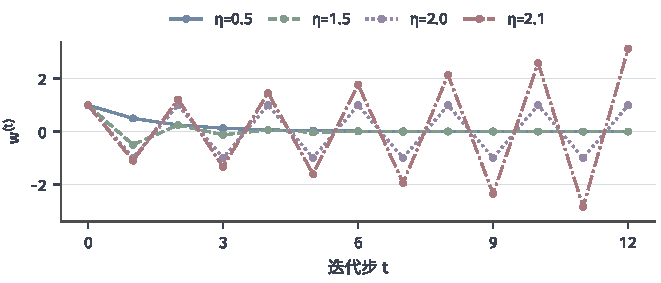
\includegraphics[width=112mm]{figures/01-mathematical-preliminaries-upper/01-mathematical-language-combinatorics-analysis-optimization/matplotlib/comprehension-additions/gradient-step-stability.pdf}
  \caption{对$f(w)=w^2/2$取$w^{(0)}=1$，画精确迭代$w^{(t)}=(1-\eta)^t$。$\eta=0.5$同侧收缩，$\eta=1.5$换侧收缩，$\eta=2$等幅振荡，$\eta=2.1$幅度增长。各点仅对应整数步，连线帮助追踪次序。这里$L=1$，稳定边界正是$2/L$。}
  \label{fig:vol1-add-gradient-step-stability}
\end{figure}

\paragraph{回溯线搜索。}
固定步长需要已知或估计$L$：估计偏大则步长过小、收敛变慢，估计偏小则下降保证失效。不依赖$L$具体数值的做法是用实际函数值检验这一步是否真的下降。给定初始试探步长$\bar\eta>0$、缩减比例$\gamma\in(0,1)$与$c\in(0,1)$，回溯线搜索从$\eta=\bar\eta$开始缩小，直到
\[
  f(\bm w-\eta\nabla f(\bm w))
  \leq f(\bm w)-c\eta\|\nabla f(\bm w)\|_2^2
\]
成立。下降引理保证$\eta\leq2(1-c)/L$时一定通过，所以全局$L$光滑时每轮有限次结束，接受步长至少为$\min\{\bar\eta,2\gamma(1-c)/L\}$。增加的成本主要是试探点函数求值。学习率调度则预先或按读数改变$\eta^{(t)}$，集中放在11.3节；两者都不能弥补错误梯度或无下界目标。

\paragraph{凸目标上的目标差。}
若$f$还凸、最小点$\bm w^\star$存在，继续取$\eta=1/L$。由凸性$f(\bm w^{(t)})-f^\star\leq\langle\nabla f(\bm w^{(t)}),\bm w^{(t)}-\bm w^\star\rangle$，结合距离平方递推和式~\eqref{eq:opt-gradient-single-step}消去梯度平方项，望远镜求和可得
\begin{equation}
  f(\bm{w}^{(T)})-f^\star
  \leq\frac{L\lVert\bm{w}^{(0)}-\bm{w}^{\star}\rVert_2^2}{2T}.
  \label{eq:opt-convex-gradient-rate}
\end{equation}

\paragraph{PL条件下的几何速度。}
\term{Polyak--Łojasiewicz条件}（PL condition）不要求函数凸，而用梯度大小控制目标差。

\begin{definition}[Polyak--Łojasiewicz条件]
\label{def:opt-pl-condition}
设$f$可微，$f^\star=\inf f>-\infty$。若存在$\mu>0$，使任意$\bm w$满足
\begin{equation}
  \frac{1}{2}\lVert\nabla f(\bm{w})\rVert_2^2
  \geq \mu\bigl(f(\bm{w})-f^{\star}\bigr),
  \label{eq:opt-pl-condition}
\end{equation}
则称$f$满足常数为$\mu$的PL条件。
\end{definition}

$\mu$强凸可微函数把式~\eqref{eq:opt-first-order-strong-convexity}右侧关于$\bm v$最小化即推出PL条件；反过来PL函数可以有多个最小点，也可以不凸。例如$f(x,y)=x^2+2\sin^2x$与$y$无关、最小点不唯一，$\partial^2 f/\partial x^2=2+4\cos2x$在某些点为负，却可验证存在$\mu>0$满足式~\eqref{eq:opt-pl-condition}。取$\eta=1/L$（必要时把常数减小到$\mu\leq L$），单步下降与PL条件给出几何收缩
\begin{equation}
  f(\bm{w}^{(t)})-f^\star
  \leq\left(1-\frac{\mu}{L}\right)^t
  \bigl(f(\bm{w}^{(0)})-f^\star\bigr).
  \label{eq:opt-pl-linear-rate}
\end{equation}
没有强凸时，这条界不保证迭代趋向某个唯一参数；已知PL常数时，$\|\nabla f\|_2\leq\sqrt{2\mu\varepsilon}$足以保证目标差不超过$\varepsilon$，但这条停止规则不能无条件用于所有光滑目标。

\paragraph{共同二次例上的逐方向核对。}
在式~\eqref{eq:opt-common-quadratic}中取$\eta=1/16$，$t\geq1$时$\bm w^{(t)}=(2(15/16)^t,0)^\top$，第二坐标一步消去，第一坐标却受较大曲率限制而缓慢缩小；$\eta=0.1$使两坐标分别乘$0.9$与$-0.6$，目标仍下降但路径振荡；$\eta=1/8$使第二坐标等幅振荡，更大则发散。一般非凸问题返回梯度范数最小的已访问点，凸问题可返回最后一点。

\subsection{固定预条件与坐标变换}

普通梯度下降用同一个标量步长，同时受陡方向的稳定限制和平坦方向的缓慢推进牵制。对固定正定矩阵$\bm P$，可以按
\begin{equation}
  \bm{w}^{(t+1)}=\bm{w}^{(t)}-\eta\bm P\nabla f(\bm{w}^{(t)})
  \label{eq:opt-fixed-precondition}
\end{equation}
重新缩放方向，这称为\term{预条件}（preconditioning）。令$\bm w=\bm P^{1/2}\bm z$，它就是新坐标下的普通梯度下降；$\bm P$不改变原目标数值，步长与停止仍按原目标选择。

对正定二次目标，变换后的曲率为$\widetilde{\bm H}=\bm P^{1/2}\bm H\bm P^{1/2}$。原坐标误差递推$(\bm I-\eta\bm P\bm H)$与新坐标递推$(\bm I-\eta\widetilde{\bm H})$相似，故特征值相同；迭代收敛当且仅当$0<\eta<2/\lambda_{\max}(\widetilde{\bm H})$，取$\eta=2/(\widetilde L+\widetilde\mu)$时每步最坏收缩因子为$(\widetilde\kappa-1)/(\widetilde\kappa+1)$，其中$\widetilde\kappa=\widetilde L/\widetilde\mu$。因此预条件的目标不是让$\bm P$自身条件数小，而是让变换后曲率$\widetilde{\bm H}$的条件数接近$1$；$\bm P$与$\bm H$不匹配时条件数反而可能增大。这一分析只针对固定$\bm P$，随历史变化的缩放矩阵必须另行说明构造与正定性。

\begin{example}[两个曲率方向上的预条件]
\label{ex:opt-anisotropic-preconditioning}
取共同二次目标、初值$(2,2)^\top$。普通梯度下降取$\eta=0.1$时两坐标分别乘以$0.9$与$-0.6$，第二坐标来回越过谷底。取$\bm P=\operatorname{diag}(1,1/16)$及$\eta=1/2$后，$\bm P\nabla f(\bm w)=\bm w$，两坐标每步都减半。
\end{example}

\begin{figure*}[htbp]
  \centering
  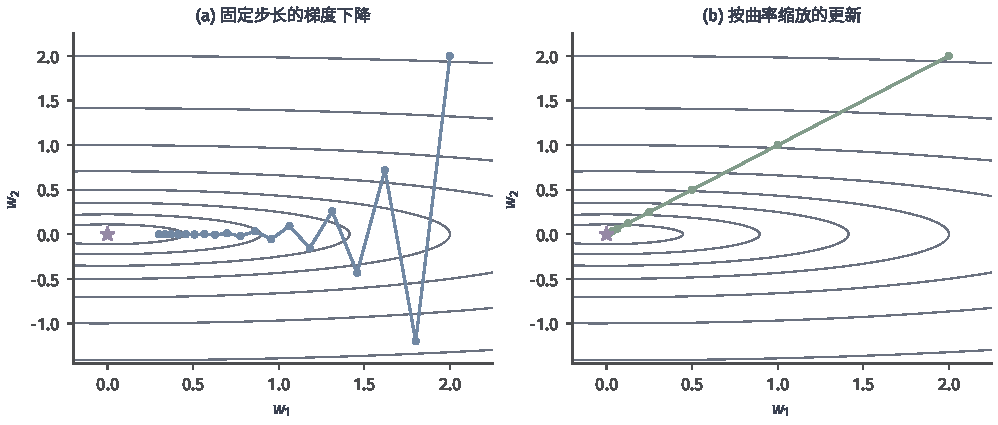
\includegraphics[width=169.0mm]{figures/01-mathematical-preliminaries-upper/01-mathematical-language-combinatorics-analysis-optimization/matplotlib/opt-preconditioned-paths/figure.pdf}
  \caption{例~\ref{ex:opt-anisotropic-preconditioning}中的精确更新路径。灰线是同一二次目标的等值线，蓝、绿圆点分别表示普通更新与预条件更新，星号是最小点。预条件使用了已知曲率，获得和应用这一矩阵的成本仍属于算法代价。}
 \label{fig:opt-preconditioned-paths}
\end{figure*}

\subsection{动量与符号方向}

这一组方法保留梯度方向或参数位移的历史。先看重球与Nesterov如何混合旧方向、在哪个点求新梯度，再看只保留符号的Lion。

\subsubsection{重球动量法}

在狭长谷底上，梯度方向在两侧之间来回摆动，真正指向谷底的分量每步却很小；想象小球在又陡又窄的滑槽里下滑，大部分动能用于撞击两壁。对连续几步指向同一侧的梯度取平均，摆动分量相消，这就是动量的作用。\term{动量法}（momentum method）的重球（heavy-ball）形式为
\[
  \bm v^{(t+1)}=\beta\bm v^{(t)}+\nabla f(\bm w^{(t)}),
  \qquad
  \bm w^{(t+1)}=\bm w^{(t)}-\eta\bm v^{(t+1)},
\]
取$\bm v^{(0)}=\bm0$启动，每轮只增加一次向量加法，不增加梯度求值。

对正定二次目标$f=\frac12\bm w^\top\bm H\bm w-\bm c^\top\bm w$，消去$\bm v$后，曲率为$\lambda_i$的特征方向上误差满足二阶递推
\[
  e_i^{(t+1)}=(1+\beta-\eta\lambda_i)e_i^{(t)}-\beta e_i^{(t-1)}.
\]
由特征多项式的Jury判据，$0\leq\beta<1$时两根都在单位圆内当且仅当$0<\eta\lambda_i<2(1+\beta)$，故所有方向稳定要求$0<\eta<2(1+\beta)/L$。已知谱界$[\mu,L]$时的经典参数为
\[
  \eta=\frac{4}{(\sqrt L+\sqrt\mu)^2},\qquad
  \beta=\left(\frac{\sqrt L-\sqrt\mu}{\sqrt L+\sqrt\mu}\right)^2,
\]
最坏方向根模至多$q=(\sqrt L-\sqrt\mu)/(\sqrt L+\sqrt\mu)$，端点重根还带来$tq^t$因子。它们是二次模型上的参数，不是一般非凸或含噪梯度下的无条件调参规则；启动阶段目标甚至可能上升——在共同二次例上取$\eta=4/25$、$\beta=9/25$，第一步目标便从$34$升至$79.2864$，之后才趋于零。

\subsubsection{Nesterov加速梯度法}

重球在当前点求梯度，其二阶递推不能直接给出一般凸目标的加速证明。\term{Nesterov加速梯度}（Nesterov accelerated gradient）改变求导位置：先外推，再在前瞻点求梯度。对凸、$L$光滑、最小点存在的目标，初始化$\bm z^{(0)}=\bm w^{(0)}$、$q^{(0)}=1$，依次计算
\begin{align*}
 \bm w^{(t+1)}&=\bm z^{(t)}-\frac1L\nabla f(\bm z^{(t)}),&
 q^{(t+1)}&=\frac{1+\sqrt{1+4(q^{(t)})^2}}2,\\
 \bm z^{(t+1)}&=\bm w^{(t+1)}
 +\frac{q^{(t)}-1}{q^{(t+1)}}(\bm w^{(t+1)}-\bm w^{(t)}).
\end{align*}
必须先得到新点，再形成下一轮前瞻点。在精确梯度与步长$1/L$下，
\begin{equation}
 f(\bm w^{(T)})-f^\star
 \leq\frac{2L\|\bm w^{(0)}-\bm w^\star\|_2^2}{(T+1)^2},
 \label{eq:opt-accelerated-finite-rate}
\end{equation}
而普通梯度下降的一般保证是$O(1/T)$。

证明用势函数把目标差与到最小点的距离合在一起。下降引理与凸性给出对任意$\bm v$成立的三点不等式
\[
 f(\bm x^+)-f(\bm v)
 \leq\frac L2\bigl(\|\bm v-\bm z\|_2^2-\|\bm v-\bm x^+\|_2^2\bigr),
 \qquad \bm x^+=\bm z-\frac1L\nabla f(\bm z).
\]
选比较点$\bm v=(1-1/q^{(t)})\bm w^{(t)}+\bm w^\star/q^{(t)}$，再用辅助点$\bm u^{(t)}$把外推位移并入同一向量，可使加权目标差与距离平方组成的量
\[
 E^{(t)}=(q^{(t-1)})^2\Delta^{(t)}
 +\frac L2\|\bm u^{(t)}-\bm w^\star\|_2^2
\]
逐步不增；启动的两次比较$E^{(1)}\leq E^{(0)}$、$E^{(2)}\leq E^{(1)}$可直接核验，一般步的衔接依赖恒等式$q^{(t)}(q^{(t)}-1)=(q^{(t-1)})^2$。由$q^{(T-1)}\geq(T+1)/2$即得式~\eqref{eq:opt-accelerated-finite-rate}。目标未必逐轮单调，一般凸情形也没有规定唯一参数；未知$L$时须配合与加速方案一致的回溯。神经网络实现中另常用固定$\beta$的前瞻变体（先令$\bar{\bm w}^{(t)}=\bm w^{(t)}-\eta_t\beta\bm m^{(t)}$，再在$\bar{\bm w}^{(t)}$求梯度更新缓冲），它与上述$q^{(t)}$方案不是同一算法，不自动继承$O(1/T^2)$界。

\subsubsection{Lion符号动量法}

若希望用历史向量形成方向、又不保留逐坐标平方统计，可以在混合梯度后只取符号。\term{Lion}取$\bm m^{(0)}=\bm0$、$\beta_1,\beta_2\in[0,1)$、$\eta_t>0$、$\lambda\geq0$，每轮先算方向$\bm z^{(t)}=\beta_1\bm m^{(t)}+(1-\beta_1)\bm g^{(t)}$，再更新并保存
\[
 \bm w^{(t+1)}=(1-\eta_t\lambda)\bm w^{(t)}
 -\eta_t\operatorname{sign}(\bm z^{(t)}),\qquad
 \bm m^{(t+1)}=\beta_2\bm m^{(t)}+(1-\beta_2)\bm g^{(t)},
\]
约定$\operatorname{sign}(\bm0)=\bm0$。方向使用旧缓冲，不能先用$\beta_2$覆盖状态。符号丢弃混合梯度的幅度：不计衰减时，若本轮有$q$个非零符号，位移范数恰为$\eta_t\sqrt q$，所以相同步长数值不代表与梯度下降或Adam相同的总位移。独立衰减项的目标解释与AdamW一样需要另行核对。

\subsection{逐坐标历史缩放}
\label{sec:opt-per-coordinate-scaling}

这一组方法按坐标记录梯度幅度，再以这些记录决定各坐标的缩放。AdaGrad累计全部历史，RMSProp改用衰减平均，AdaDelta再记录更新幅度，Adam加入方向平均，AMSGrad约束分母只增不减，AdamW把参数衰减移出统计，Adafactor压缩矩阵参数的平方表。

\subsubsection{AdaGrad}

对梯度幅度在坐标间差异明显的问题，AdaGrad累计平方梯度并按累计尺度缩放。取$\bm v^{(0)}=\bm0$、$\eta>0$、$\epsilon>0$：
\[
 \bm v^{(t+1)}=\bm v^{(t)}+\bm g^{(t)}\odot\bm g^{(t)},\qquad
 \bm w^{(t+1)}=\bm w^{(t)}
 -\frac{\eta\bm g^{(t)}}{\sqrt{\bm v^{(t+1)}}+\epsilon}.
\]
若某坐标每轮梯度同为非零$g$，忽略稳定项时第$t+1$次位移幅度约为$\eta/\sqrt{t+1}$；稀疏坐标只在实际非零时增加累计量。累计量不减，不能主动忘记早期大梯度；这里采用根号外加稳定项的版本，不与根号内加常数的实现混用。

\subsubsection{RMSProp}

为让近期梯度替换不可遗忘的累计历史，RMSProp取衰减平均：
\[
 \bm v^{(t+1)}=\rho\bm v^{(t)}+(1-\rho)\bm g^{(t)}\odot\bm g^{(t)},\qquad
 \bm w^{(t+1)}=\bm w^{(t)}
 -\eta_t\frac{\bm g^{(t)}}{\sqrt{\bm v^{(t+1)}}+\epsilon},
\]
其中$\rho\in[0,1)$。恒定坐标梯度给$\bm v^{(t+1)}=(1-\rho^{t+1})g^2$，零初始化使早期分母小于稳态；较大的$\rho$保留历史更久，也延缓响应。它只记录当前坐标系中的逐坐标幅度，不描述坐标间的耦合曲率。

\subsubsection{AdaDelta}

AdaDelta同时保存平方梯度平均$\bm v$和平方更新平均$\bm r$，取$\bm v^{(0)}=\bm r^{(0)}=\bm0$：
\[
 \bm v^{(t+1)}=\rho\bm v^{(t)}+(1-\rho)\bm g^{(t)}\odot\bm g^{(t)},
\]
\[
 \bm\Delta^{(t)}
 =-\frac{\sqrt{\bm r^{(t)}+\epsilon}}{\sqrt{\bm v^{(t+1)}+\epsilon}}
 \odot\bm g^{(t)},
\]
\[
 \bm r^{(t+1)}=\rho\bm r^{(t)}+(1-\rho)\bm\Delta^{(t)}\odot\bm\Delta^{(t)},
\]
\[
 \bm w^{(t+1)}=\bm w^{(t)}+\bm\Delta^{(t)}.
\]
分子必须用旧的$\bm r^{(t)}$，否则本步增量被循环定义；两个稳定项都在根号内，$\epsilon$还承担零状态启动作用。这里选原论文不另乘全局学习率的版本；省去独立学习率不等于省去$\rho$、$\epsilon$和初值选择。

\subsubsection{Adam}

Adam把方向平均与逐坐标幅度调整组合。取$\bm m^{(0)}=\bm v^{(0)}=\bm0$、$\beta_1,\beta_2\in[0,1)$：
\begin{align*}
 \bm m^{(t+1)}&=\beta_1\bm m^{(t)}+(1-\beta_1)\bm g^{(t)},&
 \bm v^{(t+1)}&=\beta_2\bm v^{(t)}+(1-\beta_2)\bm g^{(t)}\odot\bm g^{(t)},\\
 \widehat{\bm m}^{(t+1)}&=\frac{\bm m^{(t+1)}}{1-\beta_1^{t+1}},&
 \widehat{\bm v}^{(t+1)}&=\frac{\bm v^{(t+1)}}{1-\beta_2^{t+1}},
\end{align*}
\[
 \bm w^{(t+1)}=\bm w^{(t)}
 -\eta_t\frac{\widehat{\bm m}^{(t+1)}}{\sqrt{\widehat{\bm v}^{(t+1)}}+\epsilon}.
\]
把一阶递推展开为权重和为$1-\beta_1^{t+1}$的有限几何和，就看出偏差修正的作用：恒定梯度序列恰好恢复该梯度；这不需要概率前置，也不表示非平稳历史等于当前梯度。首步修正后非零坐标在忽略稳定项时呈符号步。历史为两组$d$维向量和步数，恢复训练须一并恢复这些状态；稳定项排除零分母，却不使方向映射自动具有统一Lipschitz常数。

正分母的连续性需要单独核验。以一个坐标的$m/(\sqrt v+\varepsilon)$为例，通分后用$|\sqrt v-\sqrt{\widetilde v}|\leq\sqrt{|v-\widetilde v|}$，方向差可由$|m-\widetilde m|/\varepsilon$与$\sqrt{|v-\widetilde v|}$的项控制；只有另有$v,\widetilde v\geq v_{\min}>0$时，才得到对$v$差的线性界。分母可算、扰动连续、统一Lipschitz是三个不同条件，不能以稳定项代替敏感度分析。

\subsubsection{AMSGrad}

Adam的平方平均会遗忘历史，分母可能回落。AMSGrad增加逐坐标历史最大值，采用不做零初始化修正的基本版本，在$\bm m,\bm v$的Adam递推之外取
\[
 \bar{\bm v}^{(t+1)}=\max(\bar{\bm v}^{(t)},\bm v^{(t+1)}),\qquad
 \bm w^{(t+1)}=\bm w^{(t)}
 -\eta_t\frac{\bm m^{(t+1)}}{\sqrt{\bar{\bm v}^{(t+1)}}+\epsilon}.
\]
逐坐标$\bar{\bm v}$不减，若$\eta_t$也不增，分母尺度对应的有效系数不增；这是代数性质，既不是目标值单调，也不是无条件的非凸收敛证明——原论文的在线凸分析另有有界域、梯度界和步长日程要求。带偏差修正的库版本须说明最大值作用在修正前还是修正后。

\subsubsection{AdamW与独立参数衰减}

若希望独立控制参数收缩、又不让衰减进入Adam的历史统计，给定数据目标$f$，仍以$\bm g^{(t)}=\nabla f(\bm w^{(t)})$执行$\bm m,\bm v$及修正，再令
\[
 \bm w^{(t+1)}=(1-\eta_t\lambda)\bm w^{(t)}
 -\eta_t\frac{\widehat{\bm m}^{(t+1)}}{\sqrt{\widehat{\bm v}^{(t+1)}}+\epsilon},
 \qquad 0\leq\eta_t\lambda<1.
\]
衰减不进入$\bm m,\bm v$，与把$\lambda\|\bm w\|_2^2/2$加到目标再运行Adam不同：后者把$\bm g+\lambda\bm w$同时送进方向与平方统计。一维首步即可复算差异：$w^0=1$、数据梯度为零、$\eta_0=0.1$、$\lambda=2$、$\epsilon=1$时，AdamW得$w^1=0.8$，对加L2目标的Adam得$14/15$。独立衰减不是固定欧氏L2目标的精确求解器；只对部分参数衰减时，所选坐标与系数必须作为算法输入给出。

\subsubsection{Adafactor}

矩阵参数的完整平方梯度表占用$O(md)$存储。Adafactor只维护行、列边际来近似它。固定参数块$\bm W^{(t)}\in\mathbb R^{m\times d}$与同点梯度$\bm D^{(t)}$，行、列状态初始为零，令$A_{ij}=(D_{ij})^2+\epsilon_1$，按
\[
 r_i^{t+1}=b_t r_i^t+(1-b_t)\frac1d\sum_jA_{ij}^t,\qquad
 c_j^{t+1}=b_t c_j^t+(1-b_t)\frac1m\sum_iA_{ij}^t
\]
更新，再重构
\[
 \widehat V_{ij}^{t+1}
 =\frac{r_i^{t+1}c_j^{t+1}}{m^{-1}\sum_k r_k^{t+1}}.
\]
同一衰减保持行列总均值一致，$\epsilon_1>0$与$b_t<1$保证重构分母为正。得到$\bm U^t=\bm D^t/\sqrt{\widehat V^{t+1}}$后，按$\operatorname{RMS}(\bm B)=\sqrt{(md)^{-1}\sum_{ij}B_{ij}^2}$把更新裁剪为$\widetilde{\bm U}^t=\bm U^t/\max\{1,\operatorname{RMS}(\bm U^t)/c_{\rm clip}\}$，取相对步长$\alpha_t=\rho_t\max\{\epsilon_2,\operatorname{RMS}(\bm W^t)\}$，令$\bm W^{t+1}=\bm W^t-\alpha_t\widetilde{\bm U}^t$。裁剪的是预条件后的更新；参数近零时$\epsilon_2$给出非零尺度。一个可执行的日程例为$b_t=1-(t+1)^{-0.8}$、$\rho_t=\min\{10^{-2},(t+1)^{-1/2}\}$。无完整动量时历史存储为$O(m+d)$，但参数、梯度和重构应用仍是$O(md)$，不能把历史节约写成整次训练只需线性存储；重构只保留行列边际，不能恢复任意单格平方历史，更不是参数Hessian。

\subsection{矩阵方向变换}

逐坐标表不能记录行列耦合；这里把已给定的梯度或动量矩阵整体作为变换对象。Shampoo依据跨步的左右Gram表缩放方向，Muon依据当步动量的奇异值结构整形方向。两者都只读取一阶信息，处理的统计也与Adafactor的逐元素平方表不同。

\subsubsection{Shampoo}

对矩阵参数$\bm W\in\mathbb R^{m\times d}$，Shampoo维护左右Gram表。取$\epsilon>0$，初始$\bm L_0=\epsilon\bm I_m$、$\bm R_0=\epsilon\bm I_d$；读取同一点的梯度$\bm D_t$后先更新
\[
 \bm L_t=\bm L_{t-1}+\bm D_t\bm D_t^\top,\qquad
 \bm R_t=\bm R_{t-1}+\bm D_t^\top\bm D_t,
\]
再用新统计形成方向
\[
 \bm W_t=\bm W_{t-1}-\eta_t\bm L_t^{-1/4}\bm D_t\bm R_t^{-1/4}.
\]
因两表正定，负四分之一次幂由正定谱分解定义，左右各用$-1/4$不能改成两次$-1/2$；它们是累计梯度Gram的矩阵函数，不是目标Hessian。两表存储为$O(m^2+d^2)$，朴素稠密求根一次约$O(m^3+d^3)$，Gram构造与双侧应用还有$O(m^2d+md^2)$成本；延迟求根会沿用旧变换，须记录刷新间隔。原文凸在线问题的遗憾界依赖凸性、尺度和轨迹距离等条件，不能迁成任意网络训练的普遍保证。

\subsubsection{Muon}

Muon先形成动量，再对动量矩阵作奇异值整形。令$\bm M_0=\bm0$、$\bm M_t=\beta\bm M_{t-1}+(1-\beta)\bm D_t$（Nesterov式分支则取$\bm H_t=(1-\beta)\bm D_t+\beta\bm M_t$，普通分支取$\bm H_t=\bm M_t$），整形后执行
\[
 \bm W_t=\bm W_{t-1}-\eta_t\kappa_{m,d}\widehat{\bm O}_t,\qquad
 \kappa_{m,d}=\sqrt{\max(1,m/d)}.
\]
理想整形的含义是：若$\bm H$有紧致奇异值分解$\bm H=\bm U_r\bm\Sigma_r\bm V_r^\top$（只保留$r$个正奇异值），理想输出为$\bm O=\bm U_r\bm V_r^\top$，即保持非零奇异子空间而把这些奇异值都变成$1$；秩亏时$\bm O\bm O^\top$、$\bm O^\top\bm O$只是相应子空间上的投影。实际实现用有限步矩阵多项式逼近：置$\bm X_0=\bm H/(\|\bm H\|_F+10^{-7})$，固定执行$K=5$次
\[
 \bm A_k=\bm X_k\bm X_k^\top,\qquad
 \bm X_{k+1}=a\bm X_k+(b\bm A_k+c\bm A_k^2)\bm X_k,
\]
\[
 (a,b,c)=(3.4445,-4.7750,2.0315),
\]
再转回原形状。有限多项式把每个奇异值$s$映成$as+bs^3+cs^5$，一般不等于精确的$\bm U_r\bm V_r^\top$，不应以“正交化”一词抹去这一区别。

对照的三阶Newton--Schulz迭代$\bm X_{k+1}=\frac32\bm X_k-\frac12(\bm X_k\bm X_k^\top)\bm X_k$从$\bm X_0=\bm H/\|\bm H\|_F$出发，正奇异值按$\varphi(s)=(3s-s^3)/2$更新，对$0<s<1$有$\varphi(s)>s$且$\varphi(s)\leq1$，故无限次精确迭代趋于把奇异值拉到$1$的$\bm U_r\bm V_r^\top$；这是极因子迭代机制的复算，不是前段有限五阶、低精度实现的误差保证。对可逆方阵，瞬时的Shampoo表达式$(\bm H\bm H^\top)^{-1/4}\bm H(\bm H^\top\bm H)^{-1/4}=\bm U\bm V^\top$恰好等于理想整形，但带历史的Shampoo与Muon并不等同；每次矩阵多项式乘法约$O(md\min(m,d))$。哪些参数矩阵交给Muon须另设参数组，作者特定训练设置的经验表现不是一般收敛结论。


\section{局部模型方法}
\label{sec:opt-second-order-methods}

一阶方法只凭梯度选方向；二阶方法在当前点构造局部二次模型，用模型给出候选位移。共同记$\bm g=\nabla f(\bm w)$、$\bm H=\nabla^2f(\bm w)$，模型为
\[
 m(\bm p)=f(\bm w)+\langle\bm g,\bm p\rangle+\frac12\bm p^\top\bm H\bm p.
\]
使用这类方法要分清四个可组合的职责：用哪种曲率（真实Hessian、正定修正、Gauss--Newton矩阵、割线近似或输出变化度量），怎样限制本轮位移（信赖域半径、立方位移正则、LM阻尼），怎样从模型求步（直接分解、矩阵向量积CG、子问题），以及怎样按原目标接受候选（线搜索、下降比值）。阻尼与AdamW的永久参数衰减是不同操作；模型在球内的全局最优也不等于原非凸目标全局最优。

\subsection{经典与阻尼牛顿法}

\term{牛顿法}（Newton's method）令模型驻点$\nabla_{\bm p}m=\bm0$，解牛顿方程
\[
 \bm H\bm p=-\bm g,\qquad
 \bm w^{+}=\bm w+\alpha\bm p.
\]
实际过程解线性方程而不显式求逆。可逆性只使方程有唯一解，$\bm H\succ\bm0$才使这个解成为二次模型的最小点并保证（非驻点时）是下降方向；Hessian不定时牛顿方向未必下降，离解较远时还需线搜索或信赖域。阻尼牛顿保持方向不变，从$\alpha=1$开始回溯，直到$f(\bm w+\alpha\bm p)\leq f(\bm w)+c\alpha\bm g^\top\bm p$（$0<c<1/2$）；正向缩步不能修复上升方向。单位步优先试探且合格即接受，才可能在解附近恢复牛顿法的快速局部收敛——永久固定$0<\alpha<1$在二次目标上只给线性收缩。

设$\nabla f(\bm w^\star)=0$，在包含$\bm w^\star$的球内$\bm H(\bm w)\succeq m\bm I$（$m>0$）且Hessian为$M$-Lipschitz。令$\bm e=\bm w-\bm w^\star$，沿线段积分梯度，单位牛顿步满足
\[
 \bm e^+=\bm H(\bm w)^{-1}\int_0^1
 \bigl(\bm H(\bm w)-\bm H(\bm w^\star+s\bm e)\bigr)\bm e\,\mathrm ds,
 \qquad
 \|\bm e^+\|_2\leq\frac{M}{2m}\|\bm e\|_2^2.
\]
初始误差足够小、使新误差仍留在同一球内时，误差逐轮平方下降，称为二次收敛。稠密问题存储Hessian需$O(d^2)$、直接分解约$O(d^3)$；共同二次例的Hessian恒定、对角，才有$O(d)$的特例成本。

\subsection{修正牛顿法}

当原Hessian奇异、不定或数值上难以使用时，先构造$\bm B=\bm H+\bm E\succ\bm0$再解$\bm B\bm p=-\bm g$，这是修正牛顿。谱移位$\bm E=\delta\bm I$与修正Cholesky是代表实现，修改的是本轮位移模型。应先核验正定与数值尺度，再求方向并对原目标线搜索；在正定解邻域应允许修正消失，以免永久移位拖慢局部过程。

修正牛顿与不精确牛顿的误差来源要分开。以$\bm p_t$为实际位移，修正模型另有$\bm B_t^{-1}\bm E_t\bm e_t$的贡献，方程残差$\bm r_t=\bm H_t\bm p_t+\bm g_t$另有$\bm H_t^{-1}\bm r_t$的贡献；二者同时存在时
\[
 \bm h_{t+1}=\bm B_t^{-1}\!\left[
 \int_0^1\bigl(\bm H_t-\bm H(\bm w^\star+s\bm h_t)\bigr)\bm h_t\,\mathrm ds
 +\bm E_t\bm h_t+\bm r_t\right].
\]
修正最终为零或$\|\bm E_t\|=O(\|\bm e_t\|)$时可保二次阶；只有$\bm E_t\to0$时结合统一逆界给超线性；永久非零移位通常留下线性项。

\subsection{信赖域方法}

二次模型只在附近可靠或曲率不定时，可以直接限制位移：在$\|\bm p\|_2\leq\Delta$内近似最小化$m(\bm p)$，这是本轮位移限制，原任务仍无约束。子问题可用Cauchy步、正定条件下的dogleg或截断CG求候选。以未加额外正则的模型下降为预报，计算
\begin{equation}
 \rho=\frac{f(\bm w)-f(\bm w+\bm p)}{m(\bm0)-m(\bm p)}.
 \label{eq:opt-trust-ratio}
\end{equation}
一种简明规则是：仅$\rho>1/4$时接受；$\rho<1/4$把半径缩为四分之一，$\rho>3/4$且步触边界时扩大两倍，其余保持；拒绝后在同一点以新半径重求。预报非正时回查内层或停止，不用零分母算比值。沿$-\bm g$在球内最小化得到Cauchy步，只要实际候选取得其固定比例的模型下降，配合目标下界、统一光滑性、模型矩阵有界和明确的接受规则，就能控制全局进展；但子问题在球内全局最小不意味着原非凸目标全局最小。

\subsection{立方正则化牛顿法}

立方正则化用Hessian的变化控制二次模型误差，求解
\[
 m_\sigma(\bm p)=m(\bm p)+\frac{\sigma}{3}\|\bm p\|^3,\qquad \sigma>0.
\]
三次项约束远处模型增长，作用于本轮位移，不等同于永久参数正则。精确模型步$\bm s$需同时满足
\[
 \bm g+\bm H\bm s+\sigma\|\bm s\|_2\bm s=\bm0,\qquad
 \bm H+\sigma\|\bm s\|_2\bm I\succeq\bm0,
\]
不能只凭模型梯度小结束。已知统一Hessian-Lipschitz常数$L_H$时取$\sigma\geq L_H/2$，三阶余项$L_H\|\bm s\|^3/6$被$\sigma\|\bm s\|^3/3$主化；未知时用ARC的比值规则按接受结果调整$\sigma$。精确全局模型步给实际下降至少$\sigma\|\bm s\|^3/6$，新点梯度为$O(\|\bm s\|^2)$，连接到一阶$O(\varepsilon^{-3/2})$的梯度评价阶；近似内层必须达到所需的下降、残差和曲率精度。

\subsection{Newton--CG与不精确牛顿法}

\subsubsection{矩阵自由求步、接受与停止}

不便形成完整Hessian时，用CG近似解$\bm H\bm p=-\bm g$，内层只调用矩阵向量积$\bm v\mapsto\bm H\bm v$。以
\[
 \|\bm H\bm p+\bm g\|_2\leq\eta_t\|\bm g\|_2,\qquad 0\leq\eta_t<1
\]
控制方程精度；这不是原目标已最优的判据。CG从零位移启动，每轮先查$\bm d_j^\top\bm H\bm d_j$，只在曲率为正时计算涉及其倒数的步长，再检查新位移是否越界：线搜索版本遇非正曲率停止并返回已得的下降方向（首内步无合格位移时回退$-\bm g$）；信赖域版本遇越界或非正曲率返回球边界步，外层仍按比值接受。内层终止的三种原因——残差满足、触边界、非正曲率——要分别记录。

\subsubsection{forcing精度与局部收敛阶}

进入非退化最小点的凸邻域后，记方程残差$\bm r_t=\bm H_t\bm p_t+\bm g_t$，用forcing参数$\vartheta_t$控制$\|\bm r_t\|_2\leq\vartheta_t\|\bm g_t\|_2$，$0\leq\vartheta_t\leq\bar\vartheta<1$。由$\bm p_t=\bm H_t^{-1}(-\bm g_t+\bm r_t)$给$\|\bm p_t\|\leq2\|\bm g_t\|/m$，对梯度作线段积分得
\begin{equation}
 \|\bm g_{t+1}\|\leq\vartheta_t\|\bm g_t\|
 +\frac{2M}{m^2}\|\bm g_t\|^2.
 \label{eq:opt-inexact-newton}
\end{equation}
固定$\vartheta_t$上界支持局部线性（在能量型范数$\|\bm h\|_*=\|\bm H_\star\bm h\|_2$下，任取$\bar\vartheta<q<1$，足够近时取得因子$q$）；$\vartheta_t\to0$给超线性；$\vartheta_t=O(\|\bm g_t\|)$给二次。固定内循环次数不自动等价于某个收敛阶。当前点的求步误差满足$\|\bm p_t-\bm p_t^N\|\leq\|\bm H_t^{-1}\|\|\bm r_t\|$，小曲率方向会放大方程残差。

\subsubsection{内层工作与外层收益}

forcing精度通常由当前梯度大小与外层阶段给定；$\vartheta_t$小往往要求更多CG迭代，但次数还取决于谱、预条件和矩阵向量积精度。远离解时二次模型不准，过度解准线性系统可能只增成本而不改善原目标，外层仍需线搜索或模型接受。

\subsection{Gauss--Newton、LM与广义Gauss--Newton法}

\subsubsection{普通Gauss--Newton法}

对非线性最小二乘$f(\bm w)=\frac12\|\bm r(\bm w)\|_2^2$，完整Hessian为
\[
 \nabla^2f=\bm J^\top\bm J+\sum_{i=1}^m r_i\nabla^2r_i,
\]
其中$\bm J$是残差Jacobian。\term{Gauss--Newton法}线性化残差、略去第二项，求解
\[
 \min_{\bm p}\frac12\|\bm r+\bm J\bm p\|_2^2,
 \qquad
 \bm J^\top\bm J\,\bm p=-\bm J^\top\bm r.
\]
$\bm J$满列秩时方向唯一；秩亏时用QR或奇异值分解取最小范数解，实践中直接解线性最小二乘而不形成平方条件数的正规方程。零残差、$\bm J$满列秩且Lipschitz、近初值时给局部二次收敛；非零残差时把更新看成迭代映射，其在解处的导数为$-(\bm J^{\star\top}\bm J^\star)^{-1}\bm E^\star$，只有该矩阵范数小于$1$才给局部线性收敛，残差大或秩条件失效时不保证收敛。

\subsubsection{Levenberg--Marquardt法}

\term{Levenberg--Marquardt法}给位移加阻尼，求
\begin{equation}
 \min_{\bm p}\frac12\|\bm r+\bm J\bm p\|_2^2+\frac{\mu}{2}\|\bm p\|_2^2,
 \qquad
 (\bm J^\top\bm J+\mu\bm I)\bm p=-\bm J^\top\bm r,
 \quad\mu>0.
 \label{eq:opt-lm-equation}
\end{equation}
\label{sec:opt-levenberg-marquardt}
即使$\bm J$秩亏，新增项也使子问题严格凸；它惩罚的是本轮位移$\bm p$，没有把原目标永久改成$f+\mu\|\bm w\|^2/2$。阻尼方程与信赖域子问题的乘子条件
\[
 (\bm J^\top\bm J+\mu\bm I)\bm p=-\bm J^\top\bm r,\quad
 \mu\geq0,\quad
 \mu(\|\bm p\|_2^2-\Delta^2)=0
\]
逐项对应；固定半径时须选择相容阻尼，不能把任意$\mu$称为该半径的精确解。

接受与否回到原目标。预报下降$\operatorname{pred}=m(\bm0)-m(\bm p)>0$时，以
\begin{equation}
 \rho=\frac{f(\bm w)-f(\bm w+\bm p)}{m(\bm0)-m(\bm p)}
 \label{eq:opt-lm-reduction-ratio}
\end{equation}
比较真实下降与模型预报，分母不含步长惩罚。取$0<\eta_a<1/4$：仅$\rho>\eta_a$接受；$\rho<1/4$把阻尼乘四，$\rho>3/4$减半，其余保持；预报非正时先增大阻尼，梯度已为零则报告驻点检查。以$r(w)=w^2-4$、$w=1/2$可完整复算：无阻尼步$p=15/4$把目标从$225/32$升到$50625/512$；$\mu=4$时步长改为$3/4$，新点$5/4$目标为$1521/512<225/32$，比值$77/48>1$，说明阻尼控制的是线性化误差而非只让方程可逆。

\subsubsection{广义Gauss--Newton法}

对一般输出损失的有限样本目标$f(\bm w)=n^{-1}\sum_i\ell_i(\bm h_i(\bm w))$，记$\bm J_i=D_{\bm w}\bm h_i$、$\bm a_i=\nabla_{\bm z}\ell_i$、$\bm S_i=\nabla_{\bm z}^2\ell_i$，链式法则给
\[
 \bm g=\frac1n\sum_i\bm J_i^\top\bm a_i,\qquad
 \bm H=\frac1n\sum_i\left[\bm J_i^\top\bm S_i\bm J_i
 +\sum_k a_{i,k}\nabla_{\bm w}^2h_{i,k}\right].
\]
广义Gauss--Newton矩阵只保留第一项$\bm G=n^{-1}\sum_i\bm J_i^\top\bm S_i\bm J_i$。若损失对输出凸则$\bm S_i\succeq\bm0$，从而$\bm G\succeq\bm0$，但复合后的$f$对参数未必凸。在当前点线性化输出、对损失保留二次项，求$(\bm G+\mu\bm I)\bm p=-\bm g$，再按原目标作Armijo接受。矩阵自由实现对$\bm v$依次算$\bm J_i\bm v$、$\bm S_i(\bm J_i\bm v)$、$\bm J_i^\top(\cdot)$即可得到$\bm G\bm v$，可回用Newton--CG接口。平方损失时$\bm S_i=\bm I$，$\bm G$退回普通GN矩阵；输出仿射时被舍项为零才有$\bm G=\bm H$。$\bm G$半正定不是原Hessian的二阶驻点证书。

\subsection{拟牛顿法：BFGS与L-BFGS}
\label{sec:opt-quasi-newton}

完整Hessian昂贵时，走过一步后已知位移与梯度变化。记
\[
 \bm s^{(t)}=\bm w^{(t+1)}-\bm w^{(t)},\qquad
 \bm y^{(t)}=\nabla f(\bm w^{(t+1)})-\nabla f(\bm w^{(t)}),
\]
沿位移积分梯度可知$\bm y^{(t)}$记录了Hessian沿该方向的平均作用；对二次目标恰有$\bm y=\bm H\bm s$。\term{拟牛顿法}要求新近似复现这一观测，即割线条件$\bm B^{(t+1)}\bm s^{(t)}=\bm y^{(t)}$。

BFGS更新保持对称，只用两个秩一项：
\begin{equation}
  \bm{B}^{(t+1)}
  =\bm{B}^{(t)}
  +\frac{\bm{y}^{(t)}(\bm{y}^{(t)})^{\top}}
         {(\bm{y}^{(t)})^{\top}\bm{s}^{(t)}}
  -\frac{\bm{B}^{(t)}\bm{s}^{(t)}(\bm{s}^{(t)})^{\top}\bm{B}^{(t)}}
         {(\bm{s}^{(t)})^{\top}\bm{B}^{(t)}\bm{s}^{(t)}}.
  \label{eq:opt-bfgs-update}
\end{equation}
当$\bm B^{(t)}\succ\bm0$且曲率条件$\bm y^\top\bm s>0$成立时，更新保持正定：对任意$\bm v\neq\bm0$展开二次型，前两项由$\bm B$内积的Cauchy--Schwarz不等式非负，仅在$\bm v\parallel\bm s$时为零，此时正曲率内积又使最后一项严格为正。沿下降方向的Wolfe线搜索保证$\bm y^\top\bm s>0$：除Armijo条件外还要求\term{Wolfe曲率条件}
\[
 \nabla f(\bm w+\alpha\bm p)^\top\bm p\geq c_2\nabla f(\bm w)^\top\bm p,
 \qquad 0<c_1<c_2<1.
\]
只缩短步长的Armijo回溯不自动满足第二式；观测曲率不可靠时可修正$\bm y$或跳过更新。

实践中维护逆近似$\bm C=\bm B^{-1}$，方向为$-\bm C\nabla f$，每轮$O(d^2)$。L-BFGS只保存最近$m$对$(\bm s_i,\bm y_i)$，用两循环递归得到方向：令$\bm q=\bm g$，从新到旧计算$\alpha_i=\rho_i\bm s_i^\top\bm q$、$\bm q\leftarrow\bm q-\alpha_i\bm y_i$；取初始尺度$\bm r=\bm C_0\bm q$（常用$\gamma\bm q$，$\gamma=\bm s^\top\bm y/\bm y^\top\bm y$），再从旧到新以$\beta_i=\rho_i\bm y_i^\top\bm r$、$\bm r\leftarrow\bm r+\bm s_i(\alpha_i-\beta_i)$恢复，$\rho_i=(\bm y_i^\top\bm s_i)^{-1}$。存储与应用成本为$O(md)$。

完整BFGS在解处Hessian正定、邻域内曲率Lipschitz、初值与初始近似足够接近、单位步优先且合格即采用等条件下超线性收敛，还要求沿实际方向的曲率逼近$|(\bm B^t-\bm H^\star)\bm p^t|/\|\bm p^t\|\to0$；每轮坚持半步虽满足Wolfe却可只线性收缩，固定记忆的L-BFGS不自动继承完整版本的超线性结论。正定二次目标上BFGS至多$d$步终止是特例，第一步并不直达最小点。

\subsection{模型变化度量：自然梯度与K-FAC}

前几种方法围绕目标函数的曲率构模；这里保持原目标不变，另用模型输出变化衡量位移。

\subsubsection{自然梯度}

给定有限输入$i=1,\ldots,n$及固定权重$\omega_i\geq0$、$\sum_i\omega_i=1$，设每个输入有$k$个正的模型输出概率$p_{ij}(\bm w)>0$、$\sum_jp_{ij}=1$，且在当前点开邻域内为$C^2$函数。定义有限对数相对变化
\[
 D_{\bm w}(\bm h)=\sum_i\omega_i\sum_j p_{ij}(\bm w)
 \log\frac{p_{ij}(\bm w)}{p_{ij}(\bm w+\bm h)}.
\]
由$-\log x\geq1-x$与归一化知$D_{\bm w}(\bm h)\geq0$。令$\bm a_{ij}=\nabla\log p_{ij}$，利用$\sum_j\nabla p_{ij}=0$与$\sum_j\nabla^2p_{ij}=0$，其二阶展开为
\[
 D_{\bm w}(\bm h)=\frac12\bm h^\top\bm F(\bm w)\bm h+o(\|\bm h\|^2),
 \qquad
 \bm F(\bm w)=\sum_{i,j}\omega_i p_{ij}\bm a_{ij}\bm a_{ij}^\top\succeq\bm0.
\]
$\bm F$未必正定（不同参数可造成相同输出变化）。给定$\bm g=\nabla f(\bm w)$，在$\bm F\succ\bm0$时，约束$\frac12\bm h^\top\bm F\bm h\leq\varepsilon$下最小化$\bm g^\top\bm h$给出自然方向$\bm h_*\propto-\bm F^{-1}\bm g$；实施时通常解阻尼系统
\[
 (\bm F+\lambda\bm I)\bm d=-\bm g,
\]
$\lambda=0$要求$\bm F\succ\bm0$，$\lambda>0$处理奇异，再按原目标回溯或给定步长更新。停止仍按原目标梯度，而非缩放后的$\|\bm d\|$。

对softmax输出与负对数似然损失，$\nabla_{\bm z}^2\ell=\operatorname{diag}(\bm p)-\bm p\bm p^\top$，此时$\bm F$正是把logit线性化所得的广义Gauss--Newton矩阵；一般目标的Hessian还含输出映射的二阶导数项。只用给定标签的对数导数外积得到的经验Fisher一般既不等于$\bm F$也不等于Hessian。一般分布的Fisher与统计几何由卷二主讲，这里不把欧氏阻尼更新宣称为精确重参数化不变。

\subsubsection{K-FAC}

完整模型度量可能难以存储求解。Kronecker分块近似曲率（K-FAC）针对矩阵参数$\bm W\in\mathbb R^{m\times d}$，把对数导数写成外积形式$\bm s_r=\bm a_r\otimes\bm\delta_r$，将块
\[
 \bm F_{\bm W}=\sum_r\pi_r\bm s_r\bm s_r^\top
 =\sum_r\pi_r(\bm a_r\bm a_r^\top\otimes\bm\delta_r\bm\delta_r^\top)
\]
近似为$\bm A\otimes\bm S$，其中
\[
 \bm A=\sum_r\pi_r\bm a_r\bm a_r^\top,\qquad
 \bm S=\sum_r\pi_r\bm\delta_r\bm\delta_r^\top.
\]
外积的加权和与两个加权和的Kronecker积一般不相等，这一步是近似而非恒等式；只配真实标签会改变外积对象。可执行的阻尼版本用（可选指数滑动的）$\bar{\bm A},\bar{\bm S}$构成$\widetilde{\bm A}=\bar{\bm A}+\lambda_A\bm I_d$、$\widetilde{\bm S}=\bar{\bm S}+\lambda_S\bm I_m$，解
\[
 \widetilde{\bm S}\bm U_t\widetilde{\bm A}=\bm D_t,
\]
再按原目标选步长。双因子阻尼对应$\widetilde{\bm A}\otimes\widetilde{\bm S}$，一般不等于$\bm F_{\bm W}+\lambda\bm I$；统计表延迟刷新时沿用旧因子，须标记统计版本。两表存储$O(m^2+d^2)$、稠密分解$O(m^3+d^3)$。

\section{步长、参数衰减与机制组合}

\subsection{学习率调度}

调度以更新时钟或指定读数产生学习率，不提供方向。约定$t=1,\ldots,T$为实际参数更新次数（梯度累积只在真正更新参数时推进$t$）。线性预热取$\eta_t=\eta_{\max}t/T_w$（$1\leq t\leq T_w$）；预热后可用分段衰减$\eta_t=\eta_{\max}\gamma^{N(t)}$（$N(t)$为已跨过的里程碑数）、指数衰减$\eta_t=\eta_{\max}\gamma^{t-T_w}$，或一次预热加余弦衰减
\[
 \eta_t=\eta_{\min}+\frac{\eta_{\max}-\eta_{\min}}2
 \left[1+\cos\!\left(\pi\frac{t-T_w}{T-T_w}\right)\right],
 \quad T_w\leq t\leq T.
\]
预热段与余弦段在$t=T_w$给出同一$\eta_{\max}$，只执行一次；$\eta_{\min}=0$时末次为零更新，不能同时声称步长严格为正。

周期重启（SGDR）为每周期保存起点与长度$T_{i+1}=qT_i$，提高学习率沿用当前参数；是否重置动量或Gram表是额外的算法选择，不由调度自动推出，也不因此获得普遍避鞍结论。指标驱动调节则每隔固定更新次数读取标量$v$，连续$p$次改善不足$\delta$时按$\eta\leftarrow\max(\eta_{\rm floor},\gamma\eta)$减小；读数来源、方向（最大化或最小化）、阈值与冷却状态都须确定，指标求值也计入预算。

\subsection{独立参数衰减}

方向形成后，还可在同一次更新中对参数施加独立衰减。先明确哪些坐标衰减、系数是否乘本次实际学习率、衰减发生在梯度进入历史统计之前还是之后。AdamW的完整更新见11.1.4.6，Lion的衰减见11.1.3.3。独立衰减与永久正则目标、硬约束半径的解对应关系在13.3.3讨论；更新中有参数收缩不等于已为某固定正则目标提供最优性证书。固定$\bm P\succ\bm0$时，对$F=f+\lambda\|\bm w\|^2/2$的参考预条件位移$\eta\bm P(\nabla f+\lambda\bm w)$与实际位移$\eta(\bm P\nabla f+\lambda\bm w)$之差为$\eta\lambda(\bm I-\bm P)\bm w$，是两种规则的确定差异，不能充作普通梯度噪声。

\subsection{执行次序、度量匹配与成本}

一条可执行的组合链必须把次序写死：在同一参数点计算原目标梯度，若用Shampoo则先更新左右Gram统计、再用新统计形成矩阵方向；随后读取调度给出的本次学习率，执行独立衰减与方向步。第14章的抽样、累积与裁剪是这条链的信息前端：在同一参数点累积读数、按声明规则裁剪，再用处理后的读数更新动量或Gram统计。先裁剪再累积、把$\lambda\bm w$加入状态更新前的梯度、把预条件方向接入不匹配度量的邻近或投影算子，得到的都是另一条算法链，不能继承原保证。每个正定变换可以在当步定义方向，但变化的度量、历史动量和延迟统计不自动满足固定矩阵下的速度条件；停止至少保留原目标认可的误差对象。

\section{收敛速度与计算复杂度}
\label{sec:opt-rates-complexity}

本节固定误差标准，比较指定算法在什么条件下需要多少迭代与计算。目标差、梯度残差和参数距离分别评价；最后一点、历史最佳点和局部邻域必须随结论注明。

\begin{table}[htbp]
 \centering\small
 \begin{tabularx}{\linewidth}{@{}lXX@{}}
 \toprule
 条件与算法 & 误差对象与返回位置 & 速度 \\
 \midrule
 凸光滑且解存在；GD／Nesterov & 最后点目标差 & $O(1/T)$／$O(1/T^2)$ \\
 光滑且满足PL；GD & 目标差 & 合格固定步长下几何收缩 \\
 光滑、目标下有界；GD & 历史最小梯度范数 & $O(\varepsilon^{-2})$次梯度迭代 \\
 Hessian-Lipschitz、下有界；精确立方全局模型步 & 新点梯度范数 & $O(\varepsilon^{-3/2})$ \\
 非退化最小点邻域；Newton／合格完整BFGS & 局部参数误差 & 二次／超线性（局部阶） \\
 \bottomrule
 \end{tabularx}
 \caption{光滑优化的代表性速度。各行的误差对象、返回位置与条件不同，不能互相套用。}
 \label{tab:opt-smooth-rates}
\end{table}

\subsection{目标值误差的收敛速度}

凸光滑且最小点存在时，距离平方递推结合凸支撑给梯度下降$O(1/T)$（式~\eqref{eq:opt-convex-gradient-rate}）；Nesterov在其完整条件下给$O(1/T^2)$（式~\eqref{eq:opt-accelerated-finite-rate}）。PL条件在$\eta=1/L$下把单步下降接成目标差的几何收缩（式~\eqref{eq:opt-pl-linear-rate}），但不要求凸或唯一解；强凸再用式~\eqref{eq:opt-strong-convex-distance}提供目标差到参数距离的控制。非凸PL反例说明不能由小梯度或局部Hessian正定直接补出全局误差保证。

\subsection{驻点残差的评价复杂度}

非凸光滑、目标下有界时，梯度下降的历史最佳残差为$O(1/\sqrt T)$，达$\varepsilon$需$O(\varepsilon^{-2})$次迭代（式~\eqref{eq:opt-nonconvex-gradient-rate}）；信赖域从模型下降、半径可靠性和接受规则连接实际下降；精确立方全局步的新点梯度为位移平方量级，给$O(\varepsilon^{-3/2})$。对正定方向尺度更新$\bm w^{t+1}=\bm w^t-\eta\bm P_t\bm g_t$，若所有$\bm P_t$对称且统一满足$m_P\bm I\preceq\bm P_t\preceq M_P\bm I$，代入光滑上界得
\[
 f(\bm w^{t+1})\leq f(\bm w^t)
 -\eta\left(m_P-\frac{L\eta M_P^2}{2}\right)\|\bm g_t\|^2,
\]
取$\eta\leq m_P/(LM_P^2)$累加给历史最小残差界；只逐轮正定而无统一界时不能写成$O(1/T)$，Adam、Lion或Muon也不能仅凭名称改写为这种$\bm P_t\bm g_t$形式。

\subsection{参数误差的局部收敛阶}

局部阶固定“已经进入非退化最小点邻域后”的参数误差，不包含到达该邻域的全程成本。单位牛顿步给二次阶$\|\bm e_{t+1}\|\leq C\|\bm e_t\|^2$，持续缩步留下未消去的一阶项；曲率修正$\bm E_t$与方程残差$\bm r_t$分别支持超线性或二次阶（11.2.5.2）；GN在零残差时二次、非零残差时条件线性；完整BFGS在严格条件下超线性，L-BFGS须另行评价。局部高阶不代表从任意初值都能进入该邻域。

\subsection{达到同一精度的总计算成本}

比较方法要同时记录外层迭代、函数／梯度／Hessian评价、分解或Hessian向量积、线搜索拒绝与存储：稠密牛顿每轮$O(d^3)$，Newton--CG每轮若做$k$次矩阵向量积为$O(kd^2)$（外加乘积本身成本），BFGS为$O(d^2)$，L-BFGS为$O(md)$，对角教学例的$O(d)$求步不代表一般二阶成本。Shampoo与K-FAC要计入Gram统计、$O(m^3+d^3)$求根和刷新频率，Muon计入固定次数的矩阵乘法；低历史存储不等于整次训练低存储。先固定同一残差或目标差标准，再合计这些工作，不能以每轮便宜单独判定总成本更低。

\section{误差传播与数值敏感度}
\label{sec:opt-numerics-sensitivity}

本节分清两个对象：固定同一目标时，初值、梯度读数、求步和舍入误差怎样沿迭代传播（算法的动态稳定性）；改变目标或数据后，最优解本身移动多少（问题的条件性）。算法快、解唯一与数值稳定不能相互代替。

\subsection{精确迭代的轨迹与稳定性}

离散梯度下降的二次特征乘子$1-\eta\lambda_i$决定同侧收缩、换号和缓慢方向；连续\term{梯度流}
\[
 \dot{\bm w}(t)=-\nabla f(\bm w(t))
\]
在假定$C^1$轨迹存在时，由链式法则$\frac{\mathrm d}{\mathrm dt}f(\bm w(t))=-\|\nabla f(\bm w(t))\|_2^2$，二次方向误差为$e_i(t)=e_i(0)e^{-\lambda_i t}$。连续流的一般存在唯一性留到微分方程章，有限步梯度下降不经误差分析不等同于连续流。动量的轨迹用11.1.3的二次递推与势函数结论比较，预条件路径要经$\bm P^{1/2}$转换再换回原坐标；各方法的逐步单调性、启动阶段和有限预算误差是不同评价对象。

\subsection{计算误差与可达到的优化精度}

把实际更新写成
\[
 \widetilde{\bm w}^{t+1}=\widetilde{\bm w}^t
 -\eta^t\bigl(\nabla F(\widetilde{\bm w}^t)+\bm e^t\bigr)+\bm u^t,
\]
其中$\bm e^t$是方向读数误差、$\bm u^t$是位移舍入；缩小步长不会以同样倍数缩小$\bm u^t$。设$F$为$L$光滑、$0<\eta^t\leq1/L$，代入下降引理并展开平方，交叉项抵消后得
\begin{equation}
 F(\widetilde{\bm w}^{t+1})
 \leq F(\widetilde{\bm w}^t)
 -\frac{\eta^t}{2}\|\nabla F(\widetilde{\bm w}^t)\|_2^2
 +\frac{\eta^t}{2}\|\bm e^t\|_2^2.
 \label{eq:opt-inexact-gradient-descent}
\end{equation}
若$F\geq F_{\inf}>-\infty$，求和给最佳驻点残差界
\begin{equation}
 \min_{t<T}\|\nabla F(\widetilde{\bm w}^t)\|^2
 \leq
 \frac{2(F(\widetilde{\bm w}^0)-F_{\inf})
 +\sum_{t<T}\eta^t\|\bm e^t\|^2}
 {\sum_{t<T}\eta^t}.
 \label{eq:opt-inexact-gradient-finite-rate}
\end{equation}
步长总和发散且加权平方误差和有限时右侧趋零；仅步长趋零不够。恒定系统偏差会留下非零误差邻域：$F(w)=w^2/2$、恒定误差$e\neq0$时轨迹趋向$-e$，目标差留在$e^2/2$。位移舍入可并入有效误差$\bm e_{\rm eff}^t=\bm e^t-\bm u^t/\eta^t$。函数值与梯度的读数误差$\tau_f,\tau_g$还要匹配接受阈值与停止残差：真实下降至少为计算下降减$2\tau_f$，$\|\widehat{\bm g}\|\leq\varepsilon$只给$\|\bm g\|\leq\varepsilon+\tau_g$。

\subsection{迭代误差的衰减、积累与放大}

理想更新映射$T^t(\bm w)=\bm w-\eta^t\nabla F(\bm w)$若有Lipschitz系数$\rho^t$，实际轨迹与理想轨迹之差$\delta^t$满足
\begin{equation}
 \delta^{t+1}\leq\rho^t\delta^t+\eta^t\|\bm e^t\|+\|\bm u^t\|,
 \label{eq:opt-inexact-gradient-recurrence}
\end{equation}
完整展开为$\delta^T\leq(\prod_{j<T}\rho^j)\delta^0+\sum_{t<T}a^t\prod_{j=t+1}^{T-1}\rho^j$。统一$\rho^t\leq\bar\rho<1$时旧误差几何衰减；只知$\rho^t\leq1$时需要注入量的一次范数可和才保证有界偏差，平方误差可和不蕴含一次范数可和：$\rho^t=1-1/(t+2)^2$的前$T$项乘积为$(T+2)/(2(T+1))\to1/2$，说明逐项小于1不等于旧误差消失。

传播系数要由目标条件取得。一般$L$光滑只给$\rho^t\leq1+\eta^tL$；增加凸性后，对$h_{\bm y}(\bm z)=F(\bm z)-\langle\nabla F(\bm y),\bm z\rangle$用下降引理可得共轭强制性
\[
 \langle\nabla F(\bm x)-\nabla F(\bm y),\bm x-\bm y\rangle
 \geq\frac1L\|\nabla F(\bm x)-\nabla F(\bm y)\|^2,
\]
故$0\leq\eta^t\leq2/L$时更新非扩张。再设$\mu\bm I\preceq\nabla^2F\preceq L\bm I$，沿线段平均Hessian给
\[
 \rho^t\leq\max\{|1-\eta^t\mu|,|1-\eta^tL|\},
\]
固定$0<\eta<2/L$才统一收缩；变步长须检查乘积。带动量或自适应统计时要把状态$\bm z^t=(\bm w^t,\bm s^t)$整体作为比较对象，Adam平方根分母的Hölder界（11.1.4.4）是构造扩展状态Lipschitz系数的依据；两条轨迹即使当前$\bm w$相同，只要动量或计时不同，下一步也可不同。样本替换的稳定性界在14.4用同一传播式建立。

\subsection{最优解对问题扰动的敏感度}

\label{sec:opt-solution-perturbation}%
固定欧氏范数和同一凸域$C$，只改变线性项：$f_{\bm b}(\bm w)=f(\bm w)-\langle\bm b,\bm w\rangle$。若$f$为$\mu$强凸，两个问题分别达到最小点$\bm w_{\bm b},\bm w_{\bm c}$，把强凸误差界分别用于两个目标和交叉候选后相加，得
\[
 \|\bm w_{\bm b}-\bm w_{\bm c}\|_2
 \leq\frac{\|\bm b-\bm c\|_2}{\mu}.
\]
被扰动的只是线性项；约束边界移动和活跃集切换不能由这个界处理（见13.8）。

对二次目标$\frac12\bm w^\top\bm H\bm w-\bm g^\top\bm w$、$\bm H\succ\bm0$，$\delta\bm w=\bm H^{-1}\delta\bm g$，故
\[
 \|\delta\bm w\|_2\leq\frac{\|\delta\bm g\|_2}{\lambda_{\min}(\bm H)}.
\]
例$f_b(w_1,w_2)=\frac12(\epsilon w_1^2+w_2^2)-bw_1$（$0<\epsilon\ll1$）的唯一解为$(b/\epsilon,0)$，$b$改变$\Delta b$时第一坐标改变$\Delta b/\epsilon$：解唯一仍可异常敏感。固定尺度的绝对放大$1/\lambda_{\min}(\bm H)$与归一化相对病态程度$\kappa(\bm H)=\lambda_{\max}/\lambda_{\min}$是两件事——$\bm H=\epsilon\bm I$条件数为$1$，绝对扰动仍放大$1/\epsilon$倍。线性空间章已证明实对称矩阵的正交谱展开与这些逆算子结论，这里只说明小曲率方向为何放大扰动，不重复证明。

\section{收敛驻点与逃离鞍点}
\label{sec:opt-stationary-saddles}

非凸光滑优化可能收敛到不是最小点的驻点。本节先固定识别依据，再比较普通梯度下降、主动扰动梯度下降和显式负曲率下降；这里分析离散迭代，连续梯度流不能代替离散算法定理。对新方法仍以原目标真梯度或曲率证书评价候选：符号输出为零、矩统计使位移很小、GGN/Fisher/Gram半正定，都不表明真实Hessian没有负曲率。

\subsection{非最小驻点与二阶证书}

内点局部最小点须满足$\bm g=\bm0$、$\bm H\succeq\bm0$，但二者不是充分条件；驻点处$\bm H\succ\bm0$是严格局部最小的充分（非必要）判据。驻点且$\lambda_{\min}(\bm H)<0$称为严格鞍点条件，该负曲率也覆盖局部极大点，不能把几何名称混同。用双容差
\[
 \|\bm g\|_2\leq\varepsilon_g,\qquad
 \lambda_{\min}(\bm H)\geq-\varepsilon_H
\]
表示近似二阶驻点；它不是一般非凸问题的最小点充分证书。精确梯度下降固定$0<\eta<2/L$时式~\eqref{eq:opt-gradient-single-step}求和给梯度平方和有限，故全部迭代的梯度范数趋零；迭代有界时至少有聚点为驻点，但不能单凭此推出整条参数序列收敛。

高阶平坦鞍点仍能通过二阶证书：全局光滑的$F(x,y)=\sin^4x-\sin^4y$在原点梯度与Hessian均为零，沿$x$轴附近目标为正、沿$y$轴为负，仍是鞍点。此处理想信赖域与立方模型步都为零，二阶证书未覆盖Hessian无负特征值的非最小驻点。

\subsection{普通GD的局部行为与渐近避鞍}

精确梯度下降从驻点出发原地不动。对更新映射$G(\bm w)=\bm w-\eta\nabla f(\bm w)$线性化，$DG(\bm w_\star)=\bm I-\eta\bm H_\star$：负特征值$-\gamma$对应放大因子$1+\eta\gamma>1$，正曲率方向在合适步长下收缩，所以偏离稳定流形的扰动可能增长，但稳定流形上的轨迹仍可趋向鞍点。例如$f(x,y)=x^4/4-x^2/2+y^2/2$从$(0,y_0)$出发、$0<\eta<2$时$x_t=0$、$y_t=(1-\eta)^ty_0$，会收敛到严格鞍点。

Lee等的固定点结论表明：$f\in C^2$、梯度全局$L$-Lipschitz、常步长$0<\eta<1/L$、初始化对Lebesgue测度绝对连续时，对每个固定严格鞍点，收敛到它的概率为零；概率只来自初始化，后续仍是确定性更新。该结论不给有限逃离步数，要称“几乎必然收敛到局部最小点”还需极限存在及所有非最小驻点都有负曲率等额外条件，也不直接适用于任意回溯步长、动量或随机梯度。

\subsection{扰动梯度下降法}

需要可量化的逃离时间时，扰动梯度下降（PGD）在可疑的小梯度区域主动加噪：正常阶段执行普通GD；当梯度小于阈值且距上次扰动满足间隔时，保存当前点$\bm z$与$f(\bm z)$，加入小球内均匀扰动，再运行规定长度的普通GD；窗口结束后若未取得规定的目标下降则返回$\bm z$，否则继续。步长、球半径、阈值、窗口按$L,L_H,\varepsilon,\delta$与初始目标差联合标定，不是任意加噪。

在$f\in C^2$、梯度$L$-Lipschitz、Hessian$L_H$-Lipschitz、目标有有限下确界等条件下，Jin等的结果以至少$1-\delta$概率返回满足
\[
 \|\nabla f(\bm w)\|_2\leq\varepsilon,\qquad
 \lambda_{\min}(\nabla^2f(\bm w))\geq-\sqrt{L_H\varepsilon}
\]
的点，梯度型迭代数为$\widetilde O(L\Delta/\varepsilon^2)$；它保证的只是近似二阶驻点，要接近局部最小点集还需定量景观条件，要全局最优还须排除坏局部最小。

\subsection{显式负曲率下降法}

若找到单位方向$\bm v$使$\bm v^\top\bm H\bm v\leq-\gamma<0$，选符号使$\bm g^\top\bm v\leq0$，在Hessian为$L_H$-Lipschitz时取$\bm s=(\gamma/L_H)\bm v$。二阶项$-\gamma\|\bm s\|^2/2$与三阶余项$L_H\|\bm s\|^3/6$合计给
\[
 f(\bm w+\bm s)-f(\bm w)\leq-\frac{\gamma^3}{3L_H^2}.
\]
即已知负曲率方向能带来可量化下降；实现先验证Rayleigh商和余项常数，再评价原目标。只要求Cauchy下降的信赖域在$\bm g=\bm0$时可能允许零步、正定修正牛顿可能返回零步、由$\bm g$启动的Newton--CG可能漏掉Krylov子空间之外的负曲率：全空间二阶证书须有相应的曲率检测与误差控制，不能仅凭CG残差小或子空间半正定出具。

\section{优化路径与隐式偏置}
\label{sec:opt-implicit-bias}

有多个最优解时算法选哪个、最优值不能在有限参数处达到时参数朝哪增长，这些由优化过程产生、未在目标中显式写出的选择偏好称为隐式偏置。本节只讨论固定有限数据上的动力学与解选择，不从训练目标或参数范数推出泛化结论；固定矩阵的几何结论不能直接扩到随历史变化的自适应统计。

\subsection{最小二乘中的初值与尺度选择}

对$F(\bm w)=\frac1{2n}\|\bm X\bm w-\bm y\|^2$，欧氏梯度$\bm X^\top(\bm X\bm w-\bm y)/n$总属于$\operatorname{range}(\bm X^\top)$，每步更新都保持$\bm w$在$\ker\bm X$上的投影；零初始化把整条轨迹限制在行空间$\operatorname{range}(\bm X^\top)=(\ker\bm X)^\perp$中。固定步长$0<\eta<2n/\|\bm X\|_2^2$时，在$\bm X^\top\bm X$特征坐标中正特征值方向的误差收缩、零特征值方向保持初值，故
\[
 \bm w^t\to\bm X^\dagger\bm y+P_{\ker X}\bm w^0,
\]
其中$\bm X^\dagger$是Moore--Penrose伪逆；零初始化的极限$\bm X^\dagger\bm y$是所有最小二乘解中欧氏范数最小者，非零初始化选择距初值最近的最小二乘解。该推导允许残差最小值非零，“插值解”只用于$\bm y\in\operatorname{range}(\bm X)$的子情形。

改为$\bm w^{t+1}=\bm w^t-\eta\bm P\nabla F(\bm w^t)$（$\bm P\succ\bm0$固定）后，令$\bm w=\bm P^{1/2}\bm v$，零初始化选择最小化$\bm w^\top\bm P^{-1}\bm w$的最小二乘解：$\bm X=(1,1)$、$\bm y=1$时，$\bm P=\bm I$给$(1/2,1/2)$，$\bm P=\operatorname{diag}(1,4)$给$(1/5,4/5)$，训练目标值同为零。尺度除影响速度外还影响欠定问题的返回解。

\subsection{可分分类中的参数发散与方向选择}

给定严格线性可分的有限数据，对无正则齐次线性预测器用logistic损失$\ell(u)=\log(1+e^{-u})$或指数损失$\ell(u)=e^{-u}$，沿任一严格分离方向放大参数即可使$F$任意接近零，但任一有限参数处$F>0$，问题没有有限最小点，应研究参数增长的方向。Soudry等在欧氏全批量梯度下降和充分小固定正步长下证明$\|\bm w^t\|\to\infty$且
\[
 \frac{\bm w^t}{\|\bm w^t\|}\longrightarrow
 \frac{\widehat{\bm w}}{\|\widehat{\bm w}\|},\qquad
 \widehat{\bm w}=\arg\min_{\bm w}\frac12\|\bm w\|^2
 \ \text{s.t.}\ y_i\bm w^\top\bm x_i\geq1\ (\forall i),
\]
即算法方向趋于硬间隔最大间隔分类器的最小范数解方向。logistic目标的全局光滑常数为$\|\bm X\|_2^2/4$；指数损失没有全局光滑常数，步长须相对数据尺度和初值选择，不能套用该常数。这是齐次线性预测器与欧氏GD的结论，改变尺度或优化方法需重新分析；损失趋零不等于参数有限收敛，也不直接给出测试误差结论。

\subsection{矩阵因子化的谱与秩选择}

$q\geq2$层因子化$\bm W=\bm W_q\cdots\bm W_1$中内部宽度$r$直接给$\operatorname{rank}(\bm W)\leq r$，这是表达限制；只有参数化容许更高秩而轨迹仍偏向某类谱结构时才谈隐式选择。对深线性网络，平衡初始化$\bm W_{j+1}(0)^\top\bm W_{j+1}(0)=\bm W_j(0)\bm W_j(0)^\top$下的梯度流在可微奇异值分支上满足$\dot s_i=-q\,s_i^{\,2-2/q}\langle\nabla f(\bm W),\bm u_i\bm v_i^\top\rangle$，幂次显示小、大奇异值的移动尺度不同，但实际增减取决于方向导数，不能仅凭幂次宣称轨迹必然最小化秩。

反例直接否定无条件的低秩倾向：对$F(\bm A,\bm B)=\frac12\|\bm A\bm B^\top-\bm I_2\|_F^2$，从$\bm A(0)=\bm B(0)=\sqrt\epsilon\bm I_2$出发梯度流保持$\bm A=\bm B=a(t)\bm I_2$，令$\lambda=a^2$则$\dot\lambda=2\lambda(1-\lambda)$，乘积矩阵始终秩为$2$、最终得到$\bm I_2$。半正定因子化的欠定插值在测量矩阵两两可交换等条件下，按“先$t\to\infty$、再初始化尺度$\alpha\downarrow0$”的顺序极限给出核范数最小解；顺序极限与可交换条件都是定理组成部分，且存在特定补全问题的反例，使因子梯度流返回秩更低却并非核范数最小的解。秩与核范数（半正定情形等于迹）是不同的量。

\subsection{非线性网络的层谱选择与边界（补充）}

两层无偏置ReLU网络中，“存在低秩插值解”不足以推出梯度流选择它：在特定的两样本、宽度$2$问题上，存在首层秩为$1$的零损失解，但当初始行、列向量范数足够小时，收敛到零损失的梯度流首层秩必为$2$。正面的深层ReLU结构结论同样带附加条件（非负标量输出、存在有界范数插值网络等），且以达到全局最小参数范数解为前提；它刻画的是层平均谱集中趋势，不证明任意梯度流达到该解。隐式偏置必须连同目标、参数化、初始化、动力学和极限对象一起陈述。

\section{本章小结}

方法主线回答能处理什么输入、改变哪个机制、怎样执行更新；性质主线按光滑性、凸性、曲率、初值和误差对象判断下降、速率与计算。方法名称不代替前提，快速局部阶不代替全程总成本：梯度历史与矩阵形状说明怎样变换方向，目标曲率和输出变化代价说明怎样建立局部模型，调度、衰减说明怎样控制整步。

数值误差可能衰减、积累或被放大，改变问题又可能移动最优解；统一收缩、精度阈值与条件数分别承担动态稳定和静态敏感度。小梯度与近似二阶驻点都不是一般非凸最小值的充分证书，渐近避鞍、高概率有限逃离和显式负曲率各有依据。优化路径还可能在多解、参数化或方向发散的任务中影响选解，最小范数、最大间隔与低秩倾向各有不同设定，不直接写成泛化保证。下一章改变可微性假设，需要为尖点重新建立可用的一阶信息与子问题。
